\documentclass[conference,10pt]{IEEEtran}
\IEEEoverridecommandlockouts
\usepackage[T1]{fontenc}
\usepackage{amsmath,amssymb}
\usepackage{graphicx}
\usepackage{booktabs}
\usepackage{multirow}
\usepackage{array}
\usepackage{xcolor}
\usepackage{tikz}
\usetikzlibrary{positioning,arrows.meta,fit,calc}
\usepackage[hidelinks]{hyperref}
\usepackage{cite}

\definecolor{ink}{HTML}{0B0B0B}
\definecolor{muted}{HTML}{52514E}
\definecolor{cblue}{HTML}{2A78D6}
\definecolor{corange}{HTML}{EB6834}
\definecolor{caqua}{HTML}{1BAF7A}
\definecolor{fblue}{HTML}{EAF2FC}
\definecolor{forange}{HTML}{FDEFE8}
\definecolor{faqua}{HTML}{E6F6EF}
\definecolor{fgray}{HTML}{F3F2EF}

\newcommand{\nat}{\textsc{nat}}
\newcommand{\syn}{\textsc{syn}}

\begin{document}

\title{Annotation-Aware WavLM Ensembles for\\Noise Event Detection in Indian Speech}

\author{\IEEEauthorblockN{Sharadh Naidu}
\IEEEauthorblockA{RV University, Bengaluru, India\\
sharadhanaidu@rvu.edu.in}
\thanks{Datathon@IndoML 2026, Track 1 (Noise Event Detection). Code, configurations, checkpoints and cached posteriors: \url{https://github.com/SharadhNaidu/noise-event-detection} (release v1.0).}}

\maketitle

\begin{abstract}
Track 1 asks for the onset and offset of every non-speech noise event in Indian-language speech recordings and scores a submission by event-level F1 plus segment-level Dice. We train frame-level taggers of six designs on 20\,ms frames. Each pairs the first four transformer layers of WavLM-Base+ with an optional AudioSet-strong BEATs stream, a bidirectional GRU, and heads for frame presence, clip presence, signed distance to the nearest boundary, and latched start/end states. The test set mixes field recordings with synthetic mixtures, which a waveform-peak test separates exactly, so each population gets its own ensemble and decoding rule. A hysteresis readout and four post-processing stages then model how annotators actually labelled the data. The final system scores 1.5926 on the leaderboard, sixth overall: F1/Dice is 0.494/0.718 on natural clips and 0.993/0.985 on synthetic ones. No external data is used. From the released posteriors the submission rebuilds with event F1 0.9996 against the uploaded file.
\end{abstract}

\section{Introduction}
The VAANI noise-event dataset~\cite{vaani_ned} annotates seven noise categories (animal, vehicle/traffic, baby/child, singing/music, phone/signal/alarm, appliance/machine, human non-speech) in speech from the VAANI corpus~\cite{vaani}. Track 1 is category-agnostic and only the time spans count. The score is $S=F_1+\mathrm{Dice}$. $F_1$ is micro-pooled over all clips with greedy one-to-one matching; a match needs both onset and offset within $\max(0.2\,d_\text{ref},50\,\text{ms})$ of the reference, where $d_\text{ref}$ is its duration~\cite{mesaros2016}. Dice is computed per clip on a 10\,ms grid and averaged over clips. Events are short (median 0.48\,s on validation, 14\% under 250\,ms) and one validation clip in eight contains overlapping events. The tolerance on a 0.48\,s event is therefore under 100\,ms, and boundary placement dominates the score. We contribute a WavLM~\cite{wavlm} frame-tagger ensemble with explicit boundary supervision, route-specific decoding, and an annotation-aware post-pass in which every stage was kept only if it improved a held-out split.

\section{Training Data and Preprocessing}
\textbf{Vaani data.} Only the official Track 1 release~\cite{vaani_ned} is used (Table~\ref{tab:data}). The human-verified tier (\emph{Gold}, 11{,}111 clips, 21.85\,h) is the core training set. From the unverified tier we keep clips whose longest event lasts at least 1.5\,s (\emph{Silver}, 12{,}014 clips), down-weighted by 0.5. The weakly labelled tier is unused. We split the 2{,}501 validation clips by speaker (SHA-256 of the speaker id, seed 42) into TUNE (1{,}257 clips) and DECIDE (1{,}244 clips), with no shared speakers. TUNE is used for training and as the noise bank below. Thresholds, ensemble composition and every post-processing stage were selected on DECIDE, which no member trains on except v5all (synthetic route only, Table~\ref{tab:mem}). \textbf{No external dataset is used}; AudioSet~\cite{audioset,audioset_strong} enters only through the pretrained BEATs weights (Table~\ref{tab:pre}).

\textbf{Preprocessing.} Audio is read with \texttt{soundfile}, averaged to mono, resampled to 16\,kHz with \texttt{librosa}, and stored as int16. Labels are rasterised to 20\,ms frames as eight channels: the union of all events (the scored target) and one channel per category. Boundary targets give each frame the signed distance to its nearest onset and offset, clipped to $\pm0.5$\,s. Models see random 5\,s crops, each z-normalised.

\textbf{Augmentation pipeline.} We build two offline synthetic stores; there is no other on-the-fly augmentation. \emph{synth\_aug} (9{,}982 clips, seed 0) has two steps. (i) A noise bank is cut from the TUNE synthetic clips as the residual \texttt{noisy}$-$\texttt{clean}, taking each labelled event $\pm$20\,ms and skipping events under 0.15\,s. (ii) Each new clip takes one of the quietest Gold hosts of at least 3\,s and inserts 1--4 bank events. Each event is resampled by a factor $\mathcal{U}(0.85,1.18)$, spectrally tilted by a one-pole filter with coefficient $\mathcal{U}(-0.6,0.6)$, and reversed with probability 0.35. It is placed uniformly at random, avoiding onsets within $\pm$50\,ms of a host event and events longer than 0.8$\times$ the host, at an SNR drawn from $\mathcal{U}(-5,15)$\,dB against the host RMS over the same span. Each clip is peak-limited to 0.99. \emph{synth\_mask\_t} (9{,}000 clips, seed 5) teaches the long, masking events common in natural recordings. A bank event is looped with 50\,ms crossfades to a duration $\mathcal{U}(2,\min(8,0.85\,d_\text{host}))$\,s, mixed into a Gold host of at least 4\,s at an SNR from $\mathcal{U}(-12,2)$\,dB, and labelled over its full extent.

\begin{table}[t]
\centering
\caption{Training stores (all from the official release).}
\label{tab:data}
\setlength{\tabcolsep}{4pt}
\footnotesize
\begin{tabular}{@{}lrl@{}}
\toprule
Store & Clips & Content and use \\
\midrule
Gold & 11{,}111 & verified timestamps, 21.85\,h; weight 1 \\
Silver & 12{,}014 & unverified tier, longest event $\geq$1.5\,s; weight 0.5 \\
TUNE & 1{,}257 & speaker-disjoint half of validation \\
synth\_aug & 9{,}982 & 1--4 bank events in Gold hosts, SNR $-5$..15\,dB \\
synth\_mask\_t & 9{,}000 & one looped 2--8\,s event, SNR $-12$..2\,dB \\
\midrule
DECIDE & 1{,}244 & held out; model and decoder selection only \\
\bottomrule
\end{tabular}
\end{table}

\begin{figure*}[t]
\centering
% Fig. 1: system overview (TikZ, full text width). Colours are defined in technical_report.tex.
\begin{tikzpicture}[font=\footnotesize, >={Stealth[length=3.6pt]}, x=0.977cm, y=0.8cm,
  box/.style={draw=muted!80, rounded corners=2.5pt, align=center, inner sep=2pt, line width=0.45pt, minimum height=0.62cm},
  arr/.style={->, draw=muted, line width=0.6pt},
  dim/.style={font=\scriptsize, text=muted, fill=white, inner sep=0.8pt},
  lab/.style={font=\scriptsize\itshape, text=muted, align=center},
  ttl/.style={font=\footnotesize\bfseries, anchor=west},
  glyph/.style={line width=0.55pt, line join=round}]
%% ---------------- (a) one member ----------------
\node[ttl] at (-0.1,4.75) {(a) One ensemble member};
% input waveform glyph
\begin{scope}[shift={(3.55,4.2)}]
  \draw[glyph, draw=ink!70] plot[smooth, samples=90, domain=-1.1:1.1] (\x, {0.17*sin(1900*\x)*exp(-2.2*(\x+0.3)^2) + 0.09*sin(3100*\x)*exp(-6*(\x-0.6)^2)});
  \node[lab, anchor=west] at (1.2,0) {5\,s crop, 16\,kHz};
\end{scope}
\node[box, fill=fblue, minimum width=3.25cm] (wav) at (1.75,3.25) {\textbf{WavLM-Base+}\\layers 1--4 (or 12, mixed)};
\node[box, fill=forange, minimum width=3.25cm] (bea) at (5.35,3.25) {\textbf{BEATs-strong} (optional)\\frozen or fine-tuned};
\draw[arr] (3.0,3.98) to[out=-150,in=90] (wav.north);
\draw[arr] (4.1,3.98) to[out=-30,in=90] (bea.north);
\node[box, fill=fgray, minimum width=6.95cm] (fus) at (3.55,2.1) {LayerNorm $\oplus$ concat (1983-d) \;$\rightarrow$\; optional Conformer (2 layers)};
\node[box, fill=fgray, minimum width=6.95cm] (gru) at (3.55,1.25) {bidirectional GRU, 2 layers $\times$ 256 per direction};
\draw[arr] (wav.south) -- (wav.south |- fus.north) node[dim, midway, right=1pt, fill=none] {$T\!\times\!768$};
\draw[arr] (bea.south) -- (bea.south |- fus.north) node[dim, midway, right=1pt, fill=none] {$T\!\times\!(768{+}447)$};
\draw[arr] (fus) -- (gru);
% heads
\foreach \x/\n/\t in {0.85/h1/frame, 2.65/h2/clip, 4.45/h3/boundary, 6.25/h4/RED latch}
  \node[box, fill=faqua, minimum width=1.62cm, minimum height=0.5cm] (\n) at (\x,0.35) {\t};
\foreach \n in {h1,h2,h3,h4} \draw[arr] (gru.south -| \n) -- (\n.north);
% head output glyphs
\begin{scope}[shift={(0.85,-0.38)}]   % frame presence, 8 tracks (one shown)
  \draw[muted!50, line width=0.3pt] (-0.7,-0.2) -- (0.7,-0.2);
  \draw[glyph, draw=cblue] plot[smooth, tension=0.5] coordinates {(-0.7,-0.18) (-0.42,-0.15) (-0.28,0.0) (-0.15,0.13) (0.05,0.1) (0.22,0.14) (0.36,-0.02) (0.5,-0.16) (0.7,-0.18)};
\end{scope}
\begin{scope}[shift={(2.65,-0.38)}]   % clip logit
  \draw[muted!50, line width=0.3pt] (-0.7,-0.2) -- (0.7,-0.2);
  \fill[cblue!80] (-0.09,-0.2) rectangle (0.09,0.15);
\end{scope}
\begin{scope}[shift={(4.45,-0.38)}]   % signed distance to nearest edge
  \draw[muted!50, line width=0.3pt] (-0.7,-0.02) -- (0.7,-0.02);
  \draw[glyph, draw=corange] (-0.7,-0.2) -- (-0.25,0.16) (-0.25,-0.2) -- (0.3,0.16) (0.3,-0.2) -- (0.7,0.1);
\end{scope}
\begin{scope}[shift={(6.25,-0.38)}]   % latched presence
  \draw[muted!50, line width=0.3pt] (-0.7,-0.2) -- (0.7,-0.2);
  \draw[glyph, draw=caqua] (-0.7,-0.2) -- (-0.3,-0.2) -- (-0.3,0.16) -- (0.35,0.16) -- (0.35,-0.2) -- (0.7,-0.2);
  \fill[ink] (-0.3,0.16) circle (0.9pt) (0.35,-0.2) circle (0.9pt);
\end{scope}
\node[lab, anchor=north] at (3.55,-0.66) {presence $\cdot$ clip score $\cdot$ signed distance to edge ($\pm$0.5\,s) $\cdot$ start/end latch};
\draw[muted!45, line width=0.4pt] (7.55,-0.95) -- (7.55,4.9);
%% ---------------- (b) inference ----------------
\node[ttl] at (7.75,4.75) {(b) Inference};
\begin{scope}[shift={(8.75,4.15)}]
  \draw[glyph, draw=ink!70] plot[smooth, samples=80, domain=-0.75:0.75] (\x, {0.15*sin(2300*\x)*exp(-3*(\x-0.15)^2)});
  \node[lab] at (0,-0.36) {test clip};
\end{scope}
\node[draw=muted!80, fill=fgray, diamond, aspect=1.5, inner sep=0.5pt, align=center, font=\scriptsize, line width=0.45pt] (route) at (8.75,2.2) {peak at\\int16 full\\scale?};
\draw[arr] (8.75,3.6) -- (route.north);
% lane geometry
\def\yn{2.95} \def\ys{0.6}


\draw[arr] (route.north east) -- ++(0.3,0.3) |- (10.05,\yn) node[pos=0.15, left, font=\scriptsize, text=muted] {yes};
\draw[arr] (route.south east) -- ++(0.3,-0.3) |- (10.05,\ys) node[pos=0.15, left, font=\scriptsize, text=muted] {no};
% ensemble boxes
\node[box, fill=fblue, minimum width=2.0cm, minimum height=1.05cm, anchor=west] (n1) at (10.05,\yn) {mean of\\7 members\\\scriptsize 3 with 3-shift TTA};
\node[box, fill=forange, minimum width=2.0cm, minimum height=1.05cm, anchor=west] (s1) at (10.05,\ys) {mean of\\6 members\\\scriptsize no TTA};
\node[font=\scriptsize\bfseries, text=cblue, anchor=south west, inner sep=1pt] at ([yshift=2pt]n1.north west) {natural recordings $\cdot$ 3{,}437 clips};
\node[font=\scriptsize\bfseries, text=corange, anchor=south west, inner sep=1pt] at ([yshift=2pt]s1.north west) {synthetic mixtures $\cdot$ 2{,}080 clips};
% readout boxes with a hysteresis glyph
\foreach \y/\n/\md in {\yn/n2/0.20, \ys/s2/0.08} {
  \node[box, fill=white, minimum width=2.75cm, minimum height=1.05cm, anchor=west] (\n) at (12.45,\y) {};
  \begin{scope}[shift={(12.6,\y-0.14)}]
    \fill[caqua!22] (0.62,0) rectangle (1.78,0.72);
    \draw[glyph, draw=cblue] plot[smooth, tension=0.6] coordinates {(0,0.08) (0.35,0.2) (0.6,0.47) (0.85,0.66) (1.05,0.58) (1.25,0.66) (1.55,0.6) (1.75,0.47) (1.92,0.25) (2.02,0.32) (2.12,0.1)};
    \draw[corange, densely dashed, line width=0.45pt] (0,0.47) -- (2.2,0.47) node[right, font=\scriptsize, text=ink, inner sep=1pt, yshift=-2pt] {.6};
    \draw[ink!80, densely dashed, line width=0.45pt] (0,0.6) -- (2.2,0.6) node[right, font=\scriptsize, text=ink, inner sep=1pt, yshift=2pt] {.7};
    \draw[muted!60, line width=0.3pt] (0,0) -- (2.2,0);
  \end{scope}
  \node[font=\scriptsize, text=muted, anchor=south, inner sep=1pt] at (13.72,\y-0.63) {min.\ \md\,s, refine};
}
\node[lab] at (11.05,\yn+1.32) {ensemble};
\node[lab] at (13.82,\yn+1.32) {hysteresis readout};
\node[lab] at (16.6,\yn+1.32) {post-pass};
% post-pass boxes
\node[box, fill=faqua, minimum width=2.4cm, minimum height=1.05cm, anchor=west, align=left, font=\scriptsize] (n3) at (15.4,\yn) {1 background extension\\2 habit full-span event\\3 nested (type-C) events};
\node[box, fill=faqua, minimum width=2.4cm, minimum height=1.05cm, anchor=west, align=left, font=\scriptsize] (s3) at (15.4,\ys) {1 level filter ($-$16\,dB)\\2 edge shift (+8/$-$6\,ms)};
\draw[arr] (n1) -- (n2); \draw[arr] (n2) -- (n3);
\draw[arr] (s1) -- (s2); \draw[arr] (s2) -- (s3);
\node[lab, anchor=north] at (13.82,-0.18) {event = maximal run with $p\geq0.6$ that reaches $p\geq0.7$ (shaded)};
\end{tikzpicture}

\caption{System overview. (a) The six members differ only in the second stream, the Conformer and the RED head (Table~\ref{tab:mem}). (b) Each test clip is routed by its waveform peak to its own ensemble, decoded by hysteresis with boundary-head refinement, and post-processed (Section~III).}
\label{fig:sys}
\end{figure*}

\section{Proposed Method}
\textbf{Architecture} (Fig.~\ref{fig:sys}a). We keep the first four of the twelve layers of WavLM-Base+~\cite{wavlm} with the convolutional front-end frozen. One member instead keeps all twelve and learns a softmax mixture of hidden states, initialised at layer 4. The optional second stream is BEATs~\cite{beats} as fine-tuned on AudioSet-strong labels by PretrainedSED~\cite{schmid2025}. It supplies a 768-d embedding plus 447 class logits per 40\,ms frame, which we upsample to 20\,ms. The stream is either precomputed and frozen or fine-tuned inside the model. Both streams are layer-normalised and concatenated (1983-d), optionally passed through a two-layer Conformer~\cite{conformer} (256-d, 4 heads, kernel 31), and fed to a two-layer BiGRU. Four heads read the GRU states. The frame head outputs eight presence logits. The clip head attention-pools a clip logit. The boundary head regresses signed seconds to the nearest onset and offset. The recurrent event detection (RED) head~\cite{schmid2026red} predicts per-frame start and end probabilities $a_t,b_t$ and decodes presence as the latch $p_t=a_t(1-p_{t-1})+(1-b_t)\,p_{t-1}$, computed with a parallel scan. Where it exists, this latch replaces the frame sigmoid at inference.

\textbf{Loss.} With $\mathcal{L}_\text{frame}$ a binary cross-entropy (positive weight 2) over all eight channels, $\mathcal{L}_\text{clip}$ the BCE against the crop maximum, and $\mathcal{L}_\text{bd}$ a Huber loss on (prediction$-$target)/50\,ms over frames within 0.5\,s of a boundary,
\begin{equation}
\mathcal{L}=\mathcal{L}_\text{frame}+0.3\,\mathcal{L}_\text{clip}+0.3\,\mathcal{L}_\text{bd}
+\big[\mathcal{L}^\text{focal}_\text{pres}+100\,(\mathcal{L}_\text{on}+\mathcal{L}_\text{off})\big]_\text{RED},
\end{equation}
where the RED terms are a focal ($\gamma\!=\!2$)~\cite{focal} presence loss and the onset/offset loss of~\cite{schmid2026red}. Clips whose events cover at least 95\% of the audio carry no frame contrast and get frame weight 0, except in members trained with whole-clip presence kept (Table~\ref{tab:mem}).

\textbf{Training.} We use AdamW~\cite{adamw} (weight decay 0.05) with a one-cycle schedule~\cite{onecycle} (15\% warm-up). Learning rates are $5\!\cdot\!10^{-5}$ for WavLM and $10^{-3}$ for the heads. In v5\_S and v12 the BEATs layers use layer-wise decay 0.8~\cite{ulmfit} from $10^{-4}$. Batches are 6 crops with 3 accumulation steps, gradients are clipped at 5, and training runs in bf16 autocast. A checkpoint is chosen by AP of the union channel minus the capped boundary error on an internal 10\% speaker-group split. Table~\ref{tab:mem} lists the members; full launch lines are recovered from the configuration stored inside each checkpoint.

\begin{table}[t]
\centering
\caption{Ensemble members (all WavLM-Base+, 5\,s crops). Params include frozen weights.}
\label{tab:mem}
\setlength{\tabcolsep}{2.6pt}
\footnotesize
\begin{tabular}{@{}lccccccc@{}}
\toprule
Member & Layers & BEATs & Conf. & RED & Ep. & Params & TTA \\
\midrule
hon\_A & 4 & -- & -- & -- & 8 & 40.4M & \checkmark \\
bts\_C & 4 & frozen & 2 & -- & 8 & 43.2M & \\
bft\_S & 4 & tuned & -- & -- & 8 & 133.3M & \checkmark \\
bts\_R & 4 & frozen & 2 & \checkmark & 8 & 43.2M & \\
v5\_S$^{\dagger}$ & 4 & tuned, LLRD & -- & \checkmark & 6 & 133.3M & \checkmark \\
v12$^{\dagger}$ & 12, mix & tuned, LLRD & -- & \checkmark & 6 & 190.0M & \\
\bottomrule
\multicolumn{8}{@{}p{0.97\columnwidth}@{}}{\scriptsize $^{\dagger}$Whole-clip presence kept. Submitted \nat\ mean: hon\_A, bts\_C, bft\_S, bts\_R, v5\_S, and two 12-layer runs (v12, seed 61; v12s62, seed 62). \syn\ mean: hon\_A, bts\_C, bft\_S, bts\_R, and v5all (the v5\_S recipe trained on all validation) counted twice.}
\end{tabular}
\end{table}

\begin{table}[t]
\centering
\caption{Pretrained models and released checkpoints.}
\label{tab:pre}
\setlength{\tabcolsep}{3pt}
\footnotesize
\begin{tabular}{@{}>{\raggedright}p{2.35cm}>{\raggedright}p{3.95cm}>{\raggedright\arraybackslash}p{1.65cm}@{}}
\toprule
Name & Source, version & Role \\
\midrule
WavLM-Base+~\cite{wavlm} & Hugging Face {\scriptsize\texttt{microsoft/wavlm-base-plus}}, revision \texttt{4c66d48} & encoder init. \\
BEATs\_strong\_1~\cite{beats} & PretrainedSED~\cite{schmid2025} v0.0.1, md5 \texttt{0b3d1253} & frame features \\
6 member checkpoints & GitHub release v1.0 (this work) & inference \\
Habit classifier & GitHub release v1.0 (this work) & post-pass \\
\bottomrule
\end{tabular}
\end{table}

\textbf{Inference and decoding} (Fig.~\ref{fig:sys}b). Posteriors are computed on 5\,s windows with a 2.5\,s hop and averaged where windows overlap. Three members also average three time shifts (zero-padding of 0, 0.64 and 1.28\,s). Natural recordings peak at int16 full scale ($\geq$32{,}765), synthetic mixtures at 0.99 of it; this rule reproduces the natural/synthetic split exactly on validation and divides the test set into 3{,}437 natural and 2{,}080 synthetic clips. Decoding uses hysteresis: an event is a maximal run of frames with $p\!\geq\!0.6$ that contains at least one frame with $p\!\geq\!0.7$, so weak bumps are rejected without shortening strong events. Events shorter than 0.2\,s (\nat) or 0.08\,s (\syn) are dropped. Gaps under 60\,ms are merged. Each edge then moves to the median of the boundary-head votes when at least three agree, by at most 0.35\,s.

\textbf{Annotation-aware post-pass.} The natural-clip stages follow labelling habits measured on validation. \emph{Background extension} lengthens events of at least 1\,s in the animal, singing/music and appliance categories while the union posterior stays above 0.3, and bridges gaps under 0.5\,s. A \emph{habit} model adds one clip-length event when annotators would likely have labelled the whole clip and no predicted event already covers 90\% of it. It is a histogram gradient-boosted classifier~\cite{sklearn} on clip-pooled BEATs tags, duration and decoder state (DECIDE AUC 0.73). \emph{Type-C} adds a category run (score $\geq$0.65, $\geq$0.3\,s) nested inside a live event at least twice as long whose dominant category differs. The scorer is category-agnostic and accepts overlapping predictions, so such nested events can still be matched. A separate overlay does the same for human non-speech inside longer events. On synthetic clips we drop events quieter than $-16$\,dB relative to the clip and shift edges by +8\,ms (onset) and $-6$\,ms (offset).

\section{Results and Conclusion}
\textbf{Leaderboard.} Table~\ref{tab:lb} and Fig.~\ref{fig:wf} trace the five submissions after the base ensemble. Every post-pass stage raised the score, and the habit stage contributed most (+0.0050, all from natural clips). The natural route is the bottleneck: synthetic clips are near ceiling (F1 0.993), whereas natural F1 is 0.494. On DECIDE, 44\% of missed natural references are covered by one prediction that spans several references, 34\% are detected with an edge outside tolerance, and 18\% are not detected. Leaderboard gains were about 0.46$\times$ the DECIDE estimates.

\begin{table}[t]
\centering
\caption{Leaderboard (test) scores per submission.}
\label{tab:lb}
\setlength{\tabcolsep}{3.2pt}
\footnotesize
\begin{tabular}{@{}lccccc@{}}
\toprule
& & \multicolumn{2}{c}{Natural} & \multicolumn{2}{c}{Synthetic} \\
\cmidrule(lr){3-4}\cmidrule(l){5-6}
Submission & Score & F1 & Dice & F1 & Dice \\
\midrule
Ensemble + readout & 1.5831 & 0.4834 & 0.7083 & -- & -- \\
+ bg.\ extension, syn.\ shift & 1.5852 & 0.4830 & 0.7096 & 0.9925 & 0.9851 \\
+ habit full-span & 1.5902 & 0.4879 & 0.7163 & 0.9925 & 0.9851 \\
+ type-C nested & 1.5907 & 0.4910 & 0.7163 & 0.9925 & 0.9851 \\
+ TTA, 2nd syn.\ shift & \textbf{1.5926} & \textbf{0.4936} & \textbf{0.7178} & \textbf{0.9929} & 0.9845 \\
\bottomrule
\multicolumn{6}{@{}l@{}}{\scriptsize Final rank: 6. The first file's synthetic split was not reported separately.}
\end{tabular}
\end{table}

\begin{figure}[t]
\centering
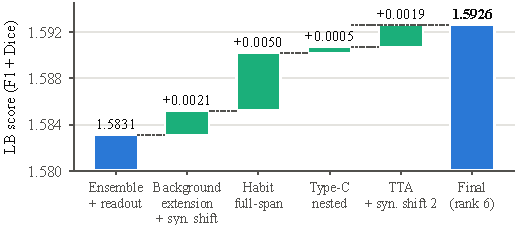
\includegraphics[width=\columnwidth]{fig/lb_waterfall.pdf}
\caption{Leaderboard gain of each post-pass stage over the base ensemble.}
\label{fig:wf}
\end{figure}

\textbf{What did not help.} Several measured negative results guided the design. Members built on stronger encoders (WavLM-Large with BEATs, Dasheng~\cite{dasheng}) were the best single models on DECIDE (1.4159 vs.\ 1.3921 for hon\_A) but lowered the ensemble by 0.008--0.010 when added to it. Global edge trimming or shifting on natural clips ($-$0.0015), a Gold-trained edge-correction CNN ($-$0.0019), duplicate events for merged references ($-$0.0035 to $-$0.0050), and test-time shifting of bts\_C ($-$0.0038) all lost on DECIDE and were not submitted.

\textbf{Reproducibility.} Rebuilding the final file from the cached posteriors and scoring it with the official scorer against the uploaded file gives F1 0.9996 and Dice 0.9993; the residue comes from three TTA posterior sets recomputed on a different GPU. Three members (v12, v12s62, v5all) were lost with a cloud instance. Live inference therefore substitutes the epoch-4 snapshot of the 12-layer run and v5\_S, and it agrees with the submitted file at F1 0.984 and Dice 0.972 (natural 0.966/0.959, synthetic 0.998/0.993). It processes the 10.8\,h test set in 66\,min on one laptop RTX 4070.

\textbf{Conclusion.} A compact WavLM ensemble with explicit boundary supervision, together with decoding and post-processing that model the annotators, reached 1.5926 and rank 6 without external data. The remaining error lies in natural recordings, where merged neighbouring events and edge placement account for most misses.

\bibliographystyle{IEEEtran}
\begin{thebibliography}{99}
\footnotesize
\bibitem{vaani_ned} P.~Kumar~J, A.~Basu, P.~Bhat, S.~Pulikodan, S.~Shukla, N.~Desai, and P.~K.~Ghosh, ``VAANI noise event dataset,'' arXiv:2609.02474, 2026; data: HF \texttt{ARTPARK-IISc/Vaani-Noise-Event-Dataset} (CC-BY-4.0).
\bibitem{vaani} S.~Pulikodan \emph{et~al.}, ``VAANI: Capturing the language landscape for an inclusive digital India,'' arXiv:2603.28714, 2026.
\bibitem{mesaros2016} A.~Mesaros, T.~Heittola, and T.~Virtanen, ``Metrics for polyphonic sound event detection,'' \emph{Appl. Sci.}, vol.~6, no.~6, p.~162, 2016.
\bibitem{wavlm} S.~Chen \emph{et~al.}, ``WavLM: Large-scale self-supervised pre-training for full stack speech processing,'' \emph{IEEE J. Sel. Topics Signal Process.}, vol.~16, no.~6, pp.~1505--1518, 2022.
\bibitem{audioset} J.~F.~Gemmeke \emph{et~al.}, ``Audio Set: An ontology and human-labeled dataset for audio events,'' in \emph{Proc. ICASSP}, 2017, pp.~776--780.
\bibitem{audioset_strong} S.~Hershey \emph{et~al.}, ``The benefit of temporally-strong labels in audio event classification,'' in \emph{Proc. ICASSP}, 2021, pp.~366--370.
\bibitem{beats} S.~Chen \emph{et~al.}, ``BEATs: Audio pre-training with acoustic tokenizers,'' in \emph{Proc. ICML}, PMLR 202, 2023, pp.~5178--5193.
\bibitem{schmid2025} F.~Schmid, T.~Morocutti, F.~Foscarin, J.~Schl\"uter, P.~Primus, and G.~Widmer, ``Effective pre-training of audio transformers for sound event detection,'' in \emph{Proc. ICASSP}, 2025.
\bibitem{conformer} A.~Gulati \emph{et~al.}, ``Conformer: Convolution-augmented transformer for speech recognition,'' in \emph{Proc. Interspeech}, 2020, pp.~5036--5040.
\bibitem{schmid2026red} F.~Schmid \emph{et~al.}, ``Sound event detection with boundary-aware optimization and inference,'' \emph{IEEE Signal Process. Lett.}, vol.~33, p.~2340, 2026.
\bibitem{focal} T.-Y.~Lin, P.~Goyal, R.~Girshick, K.~He, and P.~Doll\'ar, ``Focal loss for dense object detection,'' in \emph{Proc. ICCV}, 2017, pp.~2980--2988.
\bibitem{adamw} I.~Loshchilov and F.~Hutter, ``Decoupled weight decay regularization,'' in \emph{Proc. ICLR}, 2019.
\bibitem{onecycle} L.~N.~Smith and N.~Topin, ``Super-convergence: Very fast training of neural networks using large learning rates,'' in \emph{Proc. SPIE}, vol.~11006, 2019.
\bibitem{ulmfit} J.~Howard and S.~Ruder, ``Universal language model fine-tuning for text classification,'' in \emph{Proc. ACL}, 2018, pp.~328--339.
\bibitem{sklearn} F.~Pedregosa \emph{et~al.}, ``Scikit-learn: Machine learning in Python,'' \emph{J. Mach. Learn. Res.}, vol.~12, pp.~2825--2830, 2011.
\bibitem{dasheng} H.~Dinkel \emph{et~al.}, ``Scaling up masked audio encoder learning for general audio classification,'' in \emph{Proc. Interspeech}, 2024.
\end{thebibliography}

\end{document}
